\documentclass[11pt,a4paper]{article}

% --- Idioma y codificación ---
\usepackage[utf8]{inputenc}
\usepackage[T1]{fontenc}
\usepackage[spanish,es-noquoting]{babel}

% --- Tipografía ---
\usepackage{lmodern}
\usepackage[scaled=0.82]{beramono}
\usepackage{microtype}

% --- Página ---
\usepackage[margin=2.4cm,headsep=6mm]{geometry}
\usepackage{fancyhdr}
\usepackage{xcolor}
\usepackage{titlesec}

% --- Contenido ---
\usepackage{graphicx}
\usepackage{float}
\usepackage{caption}
\usepackage{tabularx}
\usepackage{booktabs}
\usepackage{colortbl}
\usepackage{enumitem}
\usepackage{listings}
\usepackage[hidelinks]{hyperref}

% --- Paleta ---
\definecolor{acento}{HTML}{1F3A5F}
\definecolor{gris}{HTML}{6B7280}
\definecolor{filahead}{HTML}{EEF2F7}
\definecolor{cajabg}{HTML}{F7F8FA}

% --- Títulos ---
\titleformat{\section}
  {\color{acento}\normalfont\Large\bfseries}{\thesection.}{0.6em}{}
  [\vspace{-6pt}\color{acento!30}\rule{\textwidth}{0.8pt}]
\titleformat{\subsection}
  {\color{acento!85}\normalfont\large\bfseries}{\thesubsection}{0.6em}{}
\titlespacing*{\section}{0pt}{18pt}{8pt}
\titlespacing*{\subsection}{0pt}{14pt}{6pt}

% --- Encabezado y pie ---
\pagestyle{fancy}
\fancyhf{}
\renewcommand{\headrulewidth}{0.4pt}
\renewcommand{\headrule}{\color{acento!30}\hrule height 0.4pt}
\fancyhead[L]{\small\color{gris}CC4303 Redes}
\fancyhead[R]{\small\color{gris}Construir un proxy}
\fancyfoot[C]{\small\color{gris}\thepage}

% --- Listas ---
\setlist[itemize]{itemsep=4pt, topsep=5pt, parsep=0pt, leftmargin=1.4em}

% --- Figuras ---
\captionsetup{font=small, labelfont={bf,color=acento}, skip=6pt}

% --- Bloques de código ---
\lstdefinestyle{consola}{
  basicstyle=\ttfamily\small,
  backgroundcolor=\color{cajabg},
  frame=leftline,
  framerule=2pt,
  rulecolor=\color{acento!45},
  framesep=8pt,
  xleftmargin=10pt,
  aboveskip=10pt,
  belowskip=10pt,
  breaklines=true,
  columns=fullflexible,
}
\lstset{style=consola}

\newcommand{\crlf}{\texttt{\textbackslash r\textbackslash n}}
\newcommand{\cabtabla}[1]{\rowcolor{filahead}\textbf{#1}}

\begin{document}

% --- Encabezado del documento ---
\begin{center}
{\color{acento}\LARGE\bfseries Construir un proxy\par}
\vspace{4pt}
{\large\color{gris} CC4303 Redes \textperiodcentered\ Sección Ivana Bachmann\par}
\vspace{8pt}
{Hector Bonilla V. \quad\textbullet\quad Lázaro Narváez U.\par}
\vspace{4pt}
{\small Repositorio: \url{https://github.com/LexfordMax14/redes-actividades-LN-HB}\par}
\end{center}

\vspace{6pt}
{\color{acento!30}\rule{\textwidth}{1pt}}

\section{Declaración de uso de IA}

\begin{tabularx}{\textwidth}{@{}l l X@{}}
\toprule
\cabtabla{Modelo} & \cabtabla{Integrante} & \cabtabla{Dónde se usó} \\
\midrule
Gemini & Lázaro & Consultas de sintaxis de Python sobre \texttt{.items()} y \texttt{str.replace()}.
Se usó para aprender el lenguaje y no para decisiones de diseño. \\
\addlinespace
Claude (Opus 5) & Lázaro & Diagnóstico de errores en \texttt{recive\_message} y migración del body
de \texttt{str} a \texttt{bytes}. Ejecución de las pruebas contra el servidor del curso.
Estructura de este informe. \\
\addlinespace
Claude (Sonnet) & Héctor & Consulta sobre el significado de \texttt{b\"\"} en sockets durante la
depuración de un error (la cual cierra sockets). Revisión de código. \\
\bottomrule
\end{tabularx}

\section{Cómo ejecutar}

\begin{lstlisting}
python tcp_socket_server.py
\end{lstlisting}

\begin{itemize}
  \item El programa debe ejecutarse desde la carpeta del repositorio. Los archivos
        \texttt{rules.json} y \texttt{403.jpg} se leen con ruta relativa.
  \item El proxy escucha en el puerto 8000. La dirección se define en la variable \texttt{IP\_VM}
        de \texttt{tcp\_socket\_server.py}.
  \item El comportamiento se configura en \texttt{rules.json} mediante tres campos: usuario,
        dominios bloqueados y palabras prohibidas.
\end{itemize}

\noindent Para una prueba rápida:

\begin{lstlisting}
curl http://cc4303.bachmann.cl/ -x IP_VM:8000
\end{lstlisting}

\noindent\textbf{Entorno.} El proxy fue probado en máquina virtual usando \texttt{IP\_VM} y en
localhost usando 127.0.0.1.

\section{Diagrama del proxy}

\begin{figure}[H]
  \centering
  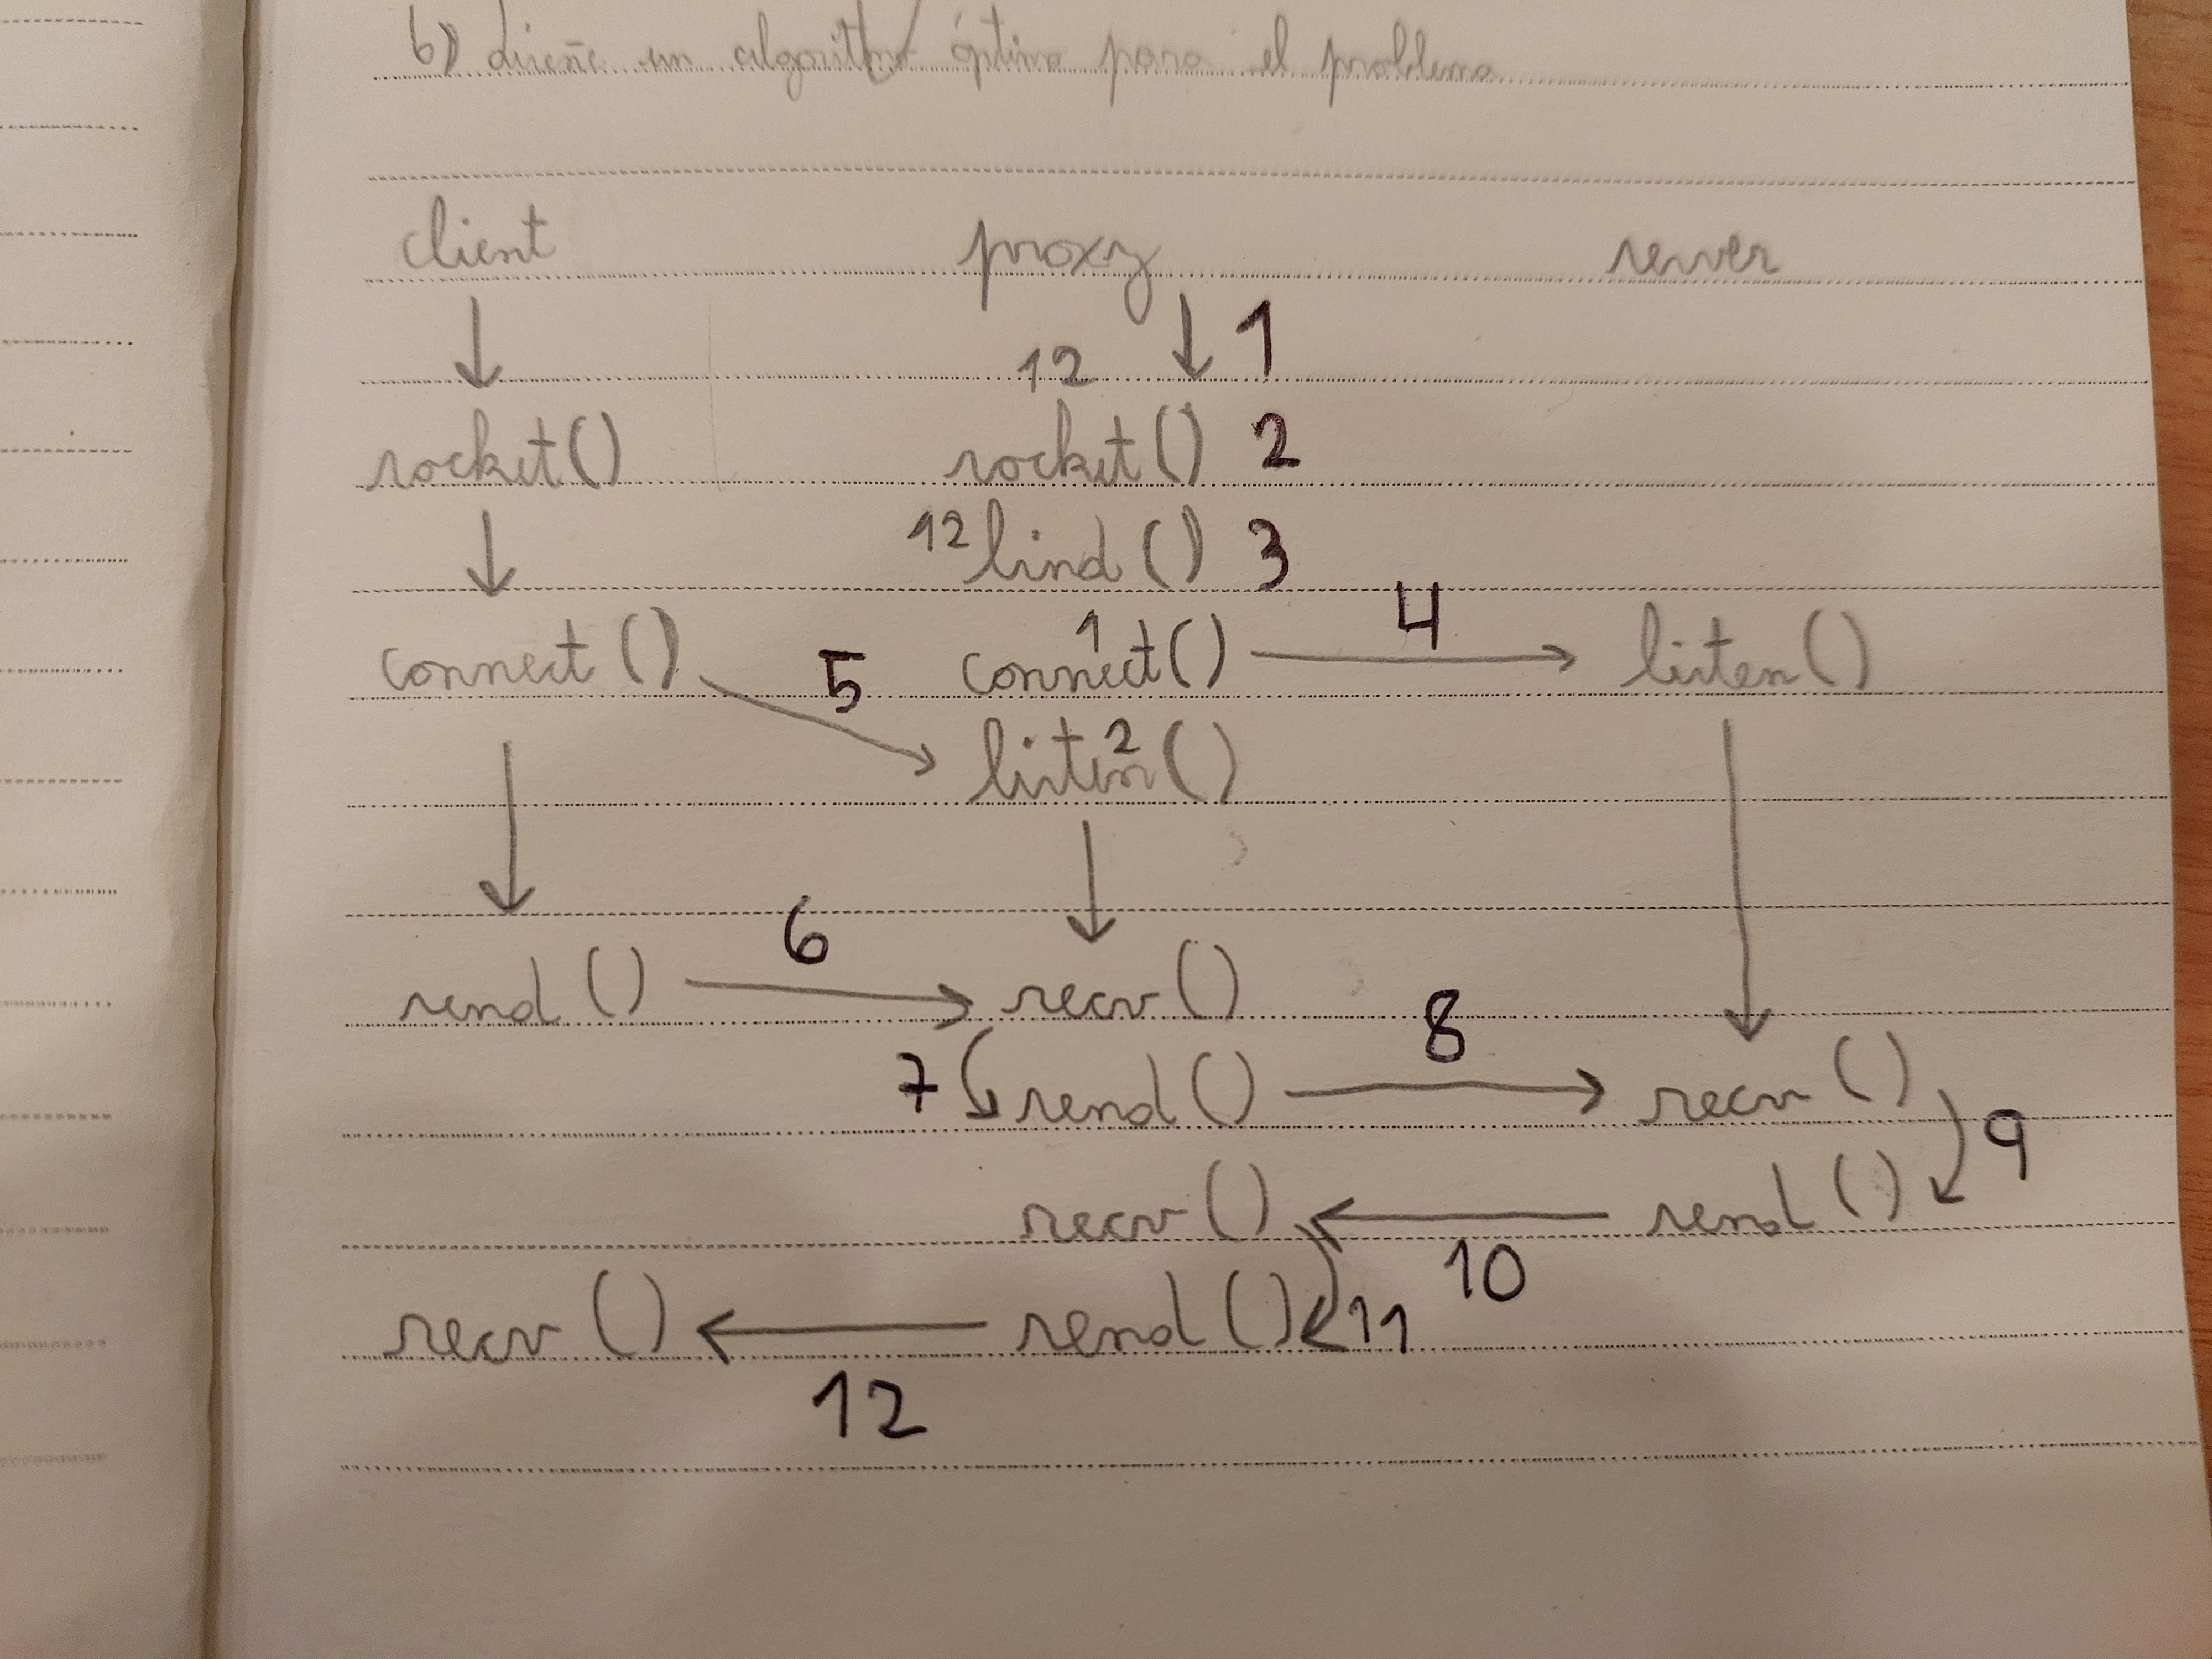
\includegraphics[width=0.95\textwidth]{diagrama.jpg}
  \caption{Flujo de llamadas entre cliente, proxy y servidor.}
\end{figure}

\noindent El proxy necesita \textbf{tres sockets} para atender una transacción.

\bigskip
\begin{tabularx}{\textwidth}{@{}l X@{}}
\toprule
\cabtabla{Socket} & \cabtabla{Rol} \\
\midrule
\texttt{server\_socket} & Recibe conexiones mediante \texttt{accept()}. No transfiere datos. \\
\addlinespace
\texttt{new\_socket}    & El proxy actúa como \textbf{servidor} frente al cliente. Se crea uno por conexión. \\
\addlinespace
\texttt{proxy\_socket}  & El proxy actúa como \textbf{cliente} frente al servidor real. \\
\bottomrule
\end{tabularx}

\bigskip
\noindent La idea central es que un proxy cumple ambos roles de forma simultánea. Recibe conexiones
con \texttt{accept()} y las origina con \texttt{connect()}.

\section{Diseño}

\subsection{Arquitectura}

\textbf{Separación en dos archivos.} El código se dividió siguiendo el principio de separación de
responsabilidades visto en Ingeniería de Software. El archivo \texttt{parser.py} implementa el
protocolo HTTP: lee del socket, interpreta mensajes y los reconstruye. El archivo
\texttt{tcp\_socket\_server.py} implementa la política del proxy: a quién conectarse, qué bloquear y
qué censurar. Ninguno de los dos necesita conocer el interior del otro.

\medskip
\noindent\textbf{Clase \texttt{Http\_HL} en lugar de un diccionario o una tupla.} Se optó por una
clase para que el editor respetara las firmas y ofreciera autocompletado. La clase además garantiza
una estructura fija donde \texttt{start\_line}, \texttt{head} y \texttt{body} siempre existen y
conservan su tipo. Esto elimina los chequeos defensivos en el resto del código.

\subsection{Qué extrae \texorpdfstring{\texttt{parse\_HTTP\_message}}{parse\_HTTP\_message}}

La función divide el mensaje en tres partes usando \crlf\crlf\ como separador.

\bigskip
\begin{tabularx}{\textwidth}{@{}l l X@{}}
\toprule
\cabtabla{Campo} & \cabtabla{Tipo} & \cabtabla{Contenido} \\
\midrule
\texttt{start\_line} & \texttt{str}            & \texttt{GET http://host/ruta HTTP/1.1}. Contiene método, path y versión \\
\texttt{head}        & \texttt{dict[str, str]} & Un par por cada header \\
\texttt{body}        & \texttt{bytes}          & Contenido crudo \\
\bottomrule
\end{tabularx}

\bigskip
\noindent Las decisiones detrás de esta estructura son dos.

\begin{itemize}
  \item \textbf{Los headers se guardan como \texttt{str} y el body como \texttt{bytes}.} La
        especificación define los headers como ASCII, mientras que el body puede ser binario como
        en el caso de un JPEG. Decodificarlo asumiendo UTF-8 provoca un error con cualquier imagen.
  \item \textbf{Se usa \texttt{partition(b":")} y no \texttt{split}.} La primera corta únicamente en
        el primer \texttt{:} del header. Esto importa porque valores como
        \texttt{Date: Thu, 27 Aug 2026 17:07:08 GMT} contienen varios.
\end{itemize}

\noindent La función \texttt{create\_HTTP\_message} es la inversa exacta. Reconstruye start line,
headers, \crlf\ y body, y devuelve el mensaje en \texttt{bytes}.

\subsection{Bloqueo de dominios}

El proxy toma la URL que el cliente escribe en la start line y verifica si alguna entrada de la
lista \texttt{blocked} aparece dentro de ella. Si aparece responde 403 y cierra la conexión. Si no,
la petición sigue por el camino normal hacia el servidor.

\begin{itemize}
  \item \textbf{Por qué se usa la start line y no el header \texttt{Host}.} El \texttt{Host} es un
        metadato del header y contiene solo el dominio, nunca lo que viene después del slash. Con él
        una entrada como \texttt{cc4303.bachmann.cl/secret} no puede calzar jamás, de modo que la
        única forma de bloquear \texttt{/secret} era bloquear el dominio completo. Eso dejaba
        inaccesibles también \texttt{/} y \texttt{/replace}. La start line en cambio trae la URL
        completa cuando el cliente pasa por un proxy, y eso permite distinguir una ruta de otra.
        Por esa razón \texttt{/replace} sigue funcionando mientras \texttt{/secret} queda bloqueado.
  \item \textbf{La comparación es por substring y no por igualdad.} La decisión es deliberada. Si
        una página está bloqueada sus rutas descendientes también deben estarlo, como ocurre con
        \texttt{/secret/algo}. El efecto lateral es que se bloquean rutas que comparten prefijo sin
        ser descendientes, por ejemplo \texttt{/secretos-publicos}. Se aceptó porque en un control
        parental resulta preferible bloquear de más que de menos.
  \item \textbf{Respuesta ante una URL bloqueada.} El proxy devuelve \texttt{403 Forbidden} junto a
        un HTML que incluye la etiqueta \texttt{<img src="/403.jpg">}.
\end{itemize}

\noindent\textbf{¿Cuántos ciclos HTTP se necesitan para mostrar una imagen en un navegador?}

\medskip
\noindent Se necesitan dos. El primero entrega el HTML y el segundo la imagen. El navegador no puede
saber que existe una imagen hasta recibir y parsear el HTML, por lo que ambas peticiones son
necesariamente secuenciales y no pueden unificarse.

\subsection{Reemplazo de palabras}

El proxy recorre \texttt{forbidden\_words}, que es una lista de diccionarios de un par cada uno, y
aplica \texttt{bytes.replace()} sobre el body por cada par. Los reemplazos son acumulativos porque
cada iteración opera sobre el resultado de la anterior.

\begin{itemize}
  \item \textbf{Se recalcula \texttt{Content-Length} tras cada reemplazo.} El body cambia de tamaño
        porque \texttt{proxy} ocupa 5 bytes y \texttt{[REDACTED]} ocupa 10. Como el body se
        almacena en \texttt{bytes}, el nuevo valor es simplemente \texttt{len(body)}. El largo debe
        medirse en bytes y no en caracteres, ya que las páginas contienen tildes.
\end{itemize}

\subsection{Modificación de headers}

El proxy agrega el header \texttt{X-ElQuePregunta} a la request que envía al servidor. Su valor se
toma de \texttt{rules.json}, lo que deja el nombre parametrizado fuera del código.

\subsection{Mensajes más grandes que el buffer}

La función \texttt{recive\_message} lee en dos fases y cada una responde a una de las preguntas
planteadas.

\medskip
\noindent\textbf{¿Cómo sé que el HEAD llegó completo?} \\
El criterio es el delimitador \crlf\crlf. La función acumula lo recibido hasta encontrarlo.

\medskip
\noindent\textbf{¿Qué pasa si los headers no caben en mi buffer?} \\
No representa un problema. La lectura no se limita a un buffer sino que acumula dentro de un
\texttt{while} hasta detectar el delimitador. El mecanismo funciona incluso con
\texttt{buff\_size=1}.

\medskip
\noindent\textbf{¿Y el BODY?} \\
El criterio es \texttt{Content-Length}. La función lee hasta que \texttt{len(body)} alcanza ese
valor.

\medskip
\noindent\textbf{¿Cómo sé si llegó el mensaje completo?} \\
Combinando ambos criterios: el delimitador para el head y \texttt{Content-Length} para el body.

\medskip
\noindent Existe un detalle que condiciona toda la implementación. Un mismo \texttt{recv} puede
traer el final del head junto con el inicio del body. Ese sobrante debe conservarse y contarse
dentro de \texttt{len(body)}. Descartarlo lleva al proxy a pedir bytes de más y quedarse bloqueado.

\medskip
\noindent\textbf{Por qué el buffer por defecto es 4 y no 50.} El valor busca forzar el peor caso en
cada ejecución. Con buffers grandes los errores de lectura no se manifiestan. Durante el desarrollo
apareció exactamente el caso descrito arriba, donde un \texttt{recv} traía el head más un fragmento
del body y ese fragmento se perdía. Con un buffer de 50 ese efecto podría no haberse observado
nunca.

\section{Pruebas}

\subsection{Con curl}

\begin{tabularx}{\textwidth}{@{}l X X@{}}
\toprule
\cabtabla{Prueba} & \cabtabla{Comando} & \cabtabla{Resultado} \\
\midrule
Bloqueo & \texttt{curl .../secret -x IP\_VM:8000} & \texttt{403} \\
\addlinespace
Imagen & \texttt{curl .../403.jpg -x IP\_VM:8000} & \texttt{200}, \texttt{image/jpeg}, 20134 bytes \\
\addlinespace
Header & \texttt{curl .../ -x IP\_VM:8000} & \texttt{Bienvenide HL!}, valor tomado de \texttt{rules.json} \\
\addlinespace
Reemplazo & \texttt{curl .../replace -x IP\_VM:8000} & 9 \texttt{[REDACTED]}, 5 \texttt{[FORBIDDEN]}
y 3 \texttt{[???]}. No queda ninguna palabra sin censurar \\
\addlinespace
Content-Length & \texttt{curl -i .../replace -x IP\_VM:8000} & El header declara 1225 bytes y el
body mide 1225 \\
\bottomrule
\end{tabularx}

\subsection{Tamaño de buffer}

Para el servidor del curso el head mide 192 bytes, la start line 17 y el mensaje completo 1351.

\bigskip
\begin{tabularx}{\textwidth}{@{}l X l@{}}
\toprule
\cabtabla{\texttt{buff\_size}} & \cabtabla{Caso} & \cabtabla{Resultado} \\
\midrule
200 & Menor que el mensaje y mayor que los headers    & Correcto \\
50  & Menor que los headers y mayor que la start line & Correcto \\
4   & Menor que la start line                         & Correcto \\
1   & Mínimo posible                                  & Correcto \\
\bottomrule
\end{tabularx}

\bigskip
\noindent En los cuatro casos el body llega completo y su largo coincide con \texttt{Content-Length}.
Los dos primeros corresponden a los escenarios exigidos por el enunciado.

\subsection{Con el navegador}

Al acceder a \texttt{http://cc4303.bachmann.cl/secret} el contenido del sitio deja de verse. El
proxy responde 403 y el navegador muestra la imagen alojada localmente. El log registra los dos
ciclos HTTP descritos antes: uno para el HTML y otro para la imagen.

\begin{figure}[H]
  \centering
  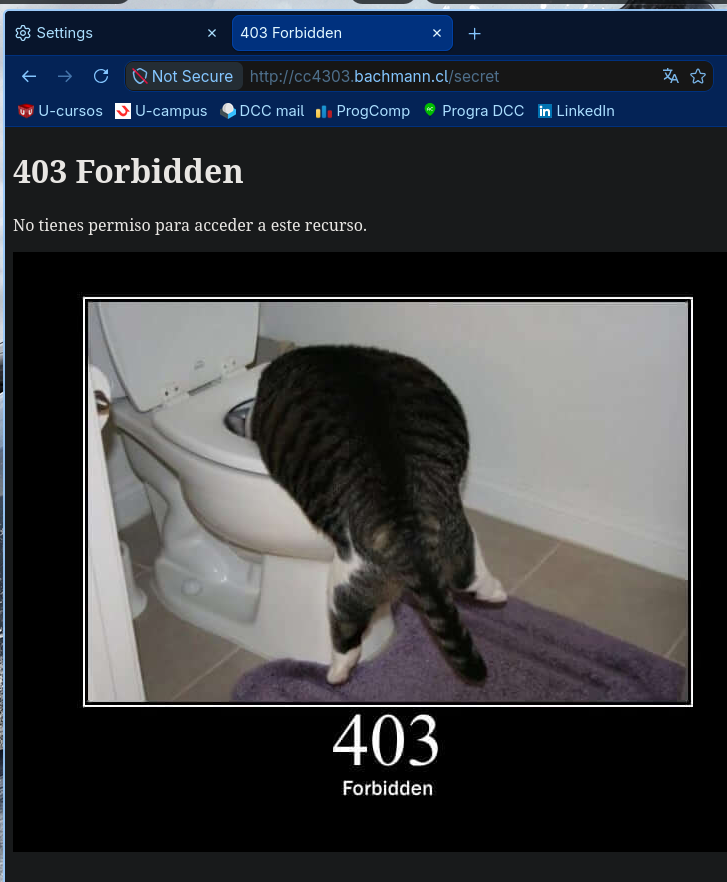
\includegraphics[width=0.62\textwidth]{secret.png}
  \caption{\texttt{/secret} bloqueado. El proxy responde 403 y sirve la imagen local.}
\end{figure}

En \texttt{http://cc4303.bachmann.cl/} el título muestra \texttt{Bienvenide HL!}. Ese valor lo toma
el servidor del header \texttt{X-ElQuePregunta} que agrega el proxy. El enlace de la página aparece
censurado.

\begin{figure}[H]
  \centering
  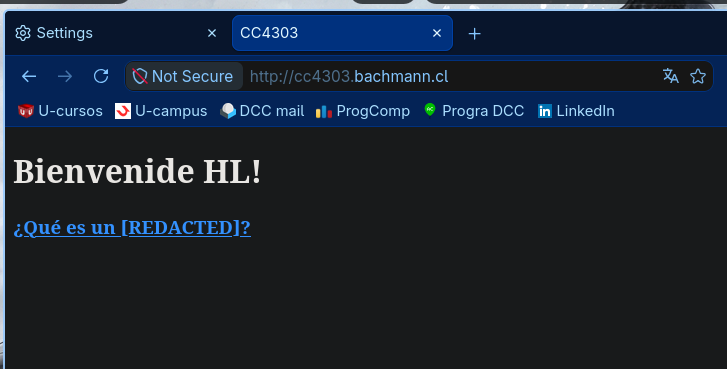
\includegraphics[width=0.92\textwidth]{root.png}
  \caption{Efecto del header \texttt{X-ElQuePregunta} sobre el mensaje de bienvenida.}
\end{figure}

En \texttt{http://cc4303.bachmann.cl/replace} el texto es el mismo que sin proxy salvo por las
palabras reemplazadas. No hay cortes ni caracteres rotos y las tildes se conservan, lo que confirma
que \texttt{Content-Length} se recalcula en bytes. El \texttt{<title>} de la pestaña también queda
censurado.

\begin{figure}[H]
  \centering
  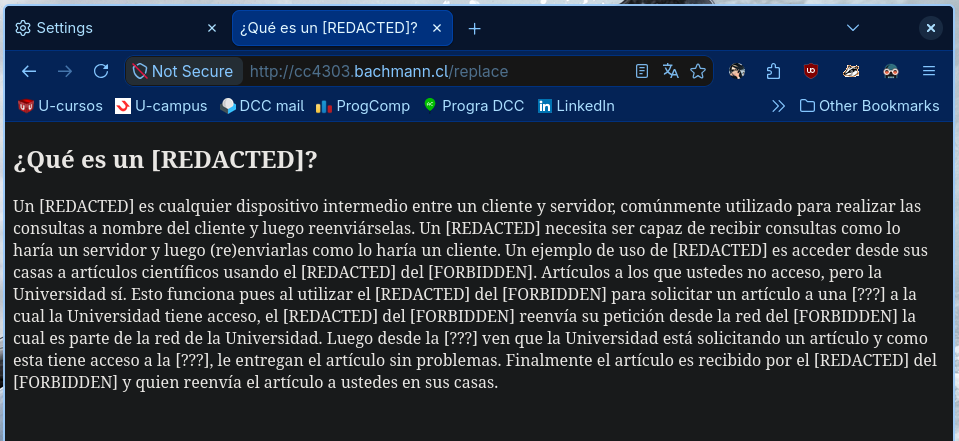
\includegraphics[width=0.92\textwidth]{replace.png}
  \caption{Palabras prohibidas censuradas en \texttt{/replace}, incluido el título de la pestaña.}
\end{figure}

\end{document}
